\chapter{\library{Lantern}: Data-driven Acoustic Echo Retrieval}\label{ch:lantern}

\marginpar{%
    \footnotesize
    \textbf{Keywords:} Acoustic Echo Retrieval, TDOA Estimation, Supervised Learning, Deep Learning, Robust Regression.
    \\\textbf{Resources:}
    \begin{itemize}
        \item \href{https://ieeexplore.ieee.org/document/8683534}{ICASSP2018 Paper}
        \item \href{https://github.com/Chutlhu/MIRAGE}{Code}
        \item \href{https://sigport.org/documents/mirage-2d-sound-source-localization-using-microphone-pair-augmentation-echoes}{ICASSP2018 Poster}
    \end{itemize}
}
\newthought{Synopsis} \synopsisChLantern

\mynewline
Deep learning notions come from readings of materials available in standard machine learning textbooks, such as~\citeonly{bishop2006pattern,goodfellow2016deep}, and the recent comprehensive work of~\citeonly{purwins2019deep} oriented towards audio signal processing.
In the remaining sections, we will present part of the previously published work~\cite{di2019mirage}, a technical report~\cite{di2019honda} and ongoing research.

\mynewline
It is essential to say that the approaches presented here are part of a first investigation in echo-aware \ac{SSL}.
Therefore they are profoundly interconnected with~\cref{ch:mirage}, which can be considered as a follow-up on the earlier work~\citeonly{gaultier2017vast} authored by colleagues.
With that being said, we will mainly focus on a simple yet common scenario where we estimate only the first and strongest echo per channel.
The generalization to multiple echoes will only be discussed as future work.

\section{Introduction}\label{sec:lantern:intro}
Recently, \acfp{DNN} have captured the attention of many research fields due to recent advances that allow for faster implementation and training, as well as for achieving considerable performance improvement.
Therefore, \acp{DNN} have been widely used in many domains.
They belong to the class of \textit{supervised} learning or \textit{data-driven} models, where the training step is performed on labeled data, namely input-output pairs.
The inclusion of these models in audio signal processing tasks has led to a considerable improvement in performance, in particular in audio and music source separation, speech enhancement, and source localization (see related sections in~\cref{ch:application}).
\\Moreover, with respect to traditional machine learning methods, the use of deep learning models presents several advantages.
They are flexible and adaptable across tasks; for instance, \acf{CNN}-based models from Computer Vision can be adapted to audio source separation (\eg/,~\citeonly{xiao2016deep, sainath2017multichannel, perotin2018crnn}), and to source localization (\eg/, ~\citeonly{chakrabarty2017broadband,vesperini2018localizing,nguyen2018autonomous,salvati2018exploiting}).
Furthermore, \acp{DNN} reduce --- even sometimes remove --- the step of designing hand-crafted features, by including feature learning as part of the learning process.
\\Other
\marginpar{
    \itshape\footnotesize
    At first, the \acf{GLLiM} framework based on \ac{GMM} was considered to address the \ac{AER} problem.
    Then, we oriented our attention towards \ac{DNN} models, which gave satisfactory results.
    It seemed that the local-linearity assumption of \ac{GLLiM} was in contrast with the highly non-linear nature of the mapping between echoes and observations.
    Nevertheless, we recognize other benefits in using the \ac{GLLiM} framework, which cannot be found in the \ac{DNN}-based approach, such as, the ability to generalize to missing data at the input or including prior statistical knowledge in the model.
} supervised learning methods have been proposed in the audio processing literature, such as \ac{GMM}-based frameworks~\citeonly{deleforge2015acoustic,gaultier2017vast}.
This framework allows to build partially informed, invertible regression models based on probabilistic prior knowledge and are competing with \ac{DNN} models in case of a small training dataset.
However, they require stronger assumptions on the nature of the mapping between input-output pairs, such as (local-)linearity or independence between variables.

\mynewline
The use of supervised learning models (not only the \acp{DNN}), presents some disadvantages.
One of the most obvious ones is their dependence on annotated data. It results in a significant bottleneck in audio signal processing tasks because collecting and annotating comprehensive real-world acoustic data is not trivial, since it requires proper tools, expertise, and time.
To overcome this issue, a standard approach nowadays is to use training data generated by simulators.
We will refer to this approach as \textit{virtually supervised learning} and it provides great versatility, for instance:
\begin{itemize}
    \item many different acoustic conditions can be include in the training data,\\\eg/, different \acf{RT$_{60}$} and \acf{SNR} levels;
    \item a precise (up to computer precision) annotation of the data is directly available,\\\eg/ spatial or temporal information on the audio scene events;
    \item and, the data can be potentially re-used for different applications,\\\eg/, localization, separation, diarization, \etc/;
\end{itemize}
Besides, the solutions obtained in a data-driven fashion suffer from bias depending on the dataset used and may not generalize to real-world scenarios.
For instance, authors of~\citeonly{deleforge2015co} showed, in a \ac{SSL} context, that training or real data collected in one part of a room and testing in another part of the same room does not generalize well.
Interestingly, the works in~\citeonly{deleforge2015acoustic,nguyen2018autonomous} propose an automatic approach for collecting and annotating data automatically as a pre-calibration step.
However, this approach is possible only with specific technologies and equipments (in both the works, the authors programmed a humanoid robot equipped with a binaural hearing system that automatically builds a training set).
The following section will give a quick overview of relevant models used in our work.

\section{Deep Learning Model}\label{sec:lantern:dnn}

\subsection{Multi-layer Perceptions}\label{subsec:lantern:mlp}
\acfp{MLP} are simple and basic modules of \acp{DNN} and are also known as \textit{fully-connected} or \textit{dense layers}.
They consist of a sequence of layers, each of which defined by an affine vector transformation followed by a an entry-wise non-linear function:
\begin{equation*}
    \bfy = f(\bfW \bfx + \bfb)
    ,
\end{equation*}
where
\newcommand{\Din}{\ensuremath{D_{\text{in}}}}
\newcommand{\Dout}{\ensuremath{D_{\text{out}}}}
\begin{itemize}
    \item $\bfx\in\bbR^{\Din}$ is the input,
    \item $\bfy\in\bbR^{\Dout}$ is the output,
    \item and $\bfb\in\bbR^{\Dout}$ and $\bfW\in\bbR^{\Dout \times \Din}$ are the \textit{bias vector} and the \textit{weight matrix}, respectively.
\end{itemize}
The function $f(\cdot)$ is a non-linear \textit{activation} function, which allows the model to learn non-linear structures.
Models built with these layers are typically used to map an input to a representation space where problems (\eg/, classification, and regression) can be addressed more easily.
The main drawback of these simple models is that they are not invariant to scaled or shifted inputs.
Since in audio data gain-, temporal-, and frequency-variations are common, they are often not suitable.
Nevertheless, \acp{MLP} are used in combination with other type of layers, such as \acfp{CNN}, \acfp{RNN}.

\newthought{Non-linear activation functions} constitute one of the key features of \acp{DNN}.
Thanks to these, the model can achieve more \textit{expressive power} with respect to linear models~\citeonly{goodfellow2016deep}.
Without these functions, it can be shown that the composition of affine transformations is equivalent to a single affine transformation.
This means that, the activation functions make the model capable of accounting for more complex relationships between the input and the output than an affine transformation.
Typical examples of these functions are the hyperbolic tangent, the Sigmoid function, and the \acf{ReLU}.

\subsection{Convolutional neural networks}\label{subsec:lantern:cnn}
The \acp{CNN} consist of convolutional layers that have been introduced to overcome some limitations of the simple linear ones.
In a nutshell, they consist of learnable kernel functions that are convolved with their input.
Therefore, they are characterized by
\begin{itemize}
    \item shift-invariance properties, thanks to the convolution operation;
    \item reduced model complexity, since the same kernel can be used at different input location;
    \item the ability to detect local structures at a different levels of abstraction in the network (see~\cref{fig:lantern:features}).
\end{itemize}
Using a Python-like notation, a 2D-convolutional layer is defined by the following equation:
\begin{equation*}
    \bfY[:,:,k] = f( \sum_{i=0}^{I-1} \bfW[:,:,i,k] \convDis \bfX[:,:,i] + \bfb[:,:,k])
    ,
\end{equation*}
where
\begin{itemize}
    \item $\bfX[:,:,i]\in\bbR^{F \times T \times I}$ and $\bfY[:,:,k]\in\bbR^{A \times B \times K}$ are input and output tensors, respectively.
    \item $i\in\klist{0,I}$ denotes the channel dimensions;\sidenote{
        In the deep learning community, input dimensions are often referred to as channels
        Based on the application, such channels \textit{do not necessarily} correspond to the channels of microphone recordings.
    }
    \item $k\in\klist{0,K}$ denotes the channel dimension in the output;
    \item the tensors $\bfW$ and $\bfb$ denotes the weight and bias tensors, respectively;
    \item $f$ is an activation function;
    \item $\convDis$ denotes discrete convolution;
\end{itemize}
A \ac{CNN} can be designed with either 1D or 2D convolutions, or a combination of them.
In general, in audio, 1D convolution layers are used to process the time-domain or frequency-domain input, whereas 2D convolutional layers are used for time-frequency representations, such as spectrograms.
The output of a convolutional layer consists of a collection of convolved versions of the input signal, which are typically referred to as \textit{feature maps}.
It is common to use \ac{CNN} architectures combining multiple convolutional layers with \textit{pooling layers} in between.
Pooling layers are used to down-sample the features maps.
In addition, to reduce the model complexity (\ie/, number of free-parameters), pooling layers subsequently reduce the size of the data as the model goes ``deeper''.
In this way, deeper layers can integrate larger extents of the data and extract spatial (in the sense of the input dimensions) features at a larger scale.
Typical pooling operators are \textit{max-pooling} and \textit{mean-pooling}, which samples non-overlapping patches by keeping the largest and the average value in the region, respectively.

\subsection{Hybrid architectures}
As mentioned earlier, modern \ac{DNN} architectures consist of a combination of different types of layers.
For instance, \acp{CNN} are used to overcome the lack of shift and scale invariance that \acp{MLP} suffer from, and allow to the extract of spatial features.
In contrast, \acp{MLP} offer a simple and generic mappings from high-dimensional spaces to lower ones, suitable for classification and regression problems.
Therefore, hybrid architectures are now the standard for deep learning models.

\subsection{Learning and optimization}
\newcommand{\params}{\ensuremath{\boldsymbol{\theta}}}
A \ac{DNN} model consists of thousands of parameters $\params$.
In order to learn a specific task, such as regression or classification, they need to be optimized.
To optimize the parameters $\params$, a variant of the gradient descent algorithm is usually implemented.
A \textit{loss function} $\calL_{\params}(\hat{\bfY},\bfY)$ measure the difference between the predicted values $\hat{\bfY}$ and the desired ones $\bfY$.
The optimization process then iteratively updates the parameters $\params$ so the loss function is minimized.
In the case of vanilla gradient descent this writes:
\begin{equation*}
    \params \gets \params - \eta \knabla_{\params} \calL_{\params}(\hat{\bfY},\bfY)
    ,
\end{equation*}
where $\eta$ is referred to as the \textit{learning rate} and controls the length of the \textit{gradient step} at each iteration.
Due to the composite structure of the \acp{DNN}, the gradient $\knabla_{\params} \calL_{\params}(\hat{\bfY},\bfY)$ is computed via the chain rule, using the \textit{back propagation} algorithm.
Most gradient descent variants used today adapt the learning rate along iterations, such as the popular \textit{Adam optimizer}~\citeonly{kingma2014adam}.
\\The \textit{Stochastic Gradient Descent} is a variant of the gradient descent algorithm which has become the standard for training \acp{DNN} today.
It was introduced to improve convergence and to solve computational and memory load issues occurring when using training sets.
It approximates the gradient at each step on a mini-bach of data samples.
Finally, we would like to mention the following common techniques used to avoid overfitting and speed up the convergence.
\begin{itemize}
    \item \textit{early stopping} allows to stop the training upon some conditions on the loss function (or other metrics), for instance, when it is not improving after certain amount of iterations.
    This criteria is typically computed on a dedicated data set known as \textit{validation} set to avoid overfitting;
    \item \textit{batch normalization} consists of scaling the data by estimating their statistics during training, which usually leads to better performance and faster convergence;
    \item \textit{dropout} is a regularization technique that reduces overfitting by randomly omitting some network units during training.
\end{itemize}

% \subsection{End-to-end and Hybrid approaches}
% The general scheme of \ac{DNN}-based approaches its one of the reasons for their success.
% Therefore they have been applied to solve many problems and at a different level of complexity.
% We can then identify to main tendencies in signal processing: end-to-end and hybrids approaches. The former attempts to address signal processing problems by getting rid of signal processing entirely as opposed to the latter.
% Although end-to-end architecture performs only marginally better than hybrid or other models, it is a common belief that soon they will outperform them~\citeonly[Chapter 19]{vincent2018audio}.

\mynewline
In this chapter, we will propose a framework based on the following hybrid approach:
we will use \ac{DNN} to estimate echoes' properties, and later, in~\cref{ch:mirage}, we will use such quantities to address \ac{SSL} problem.

\section{Learning the first echo}\label{sec:lantern:simple}

\subsection{Scenario and motivations}
\marginpar{%
    \centering
    \footnotesize
    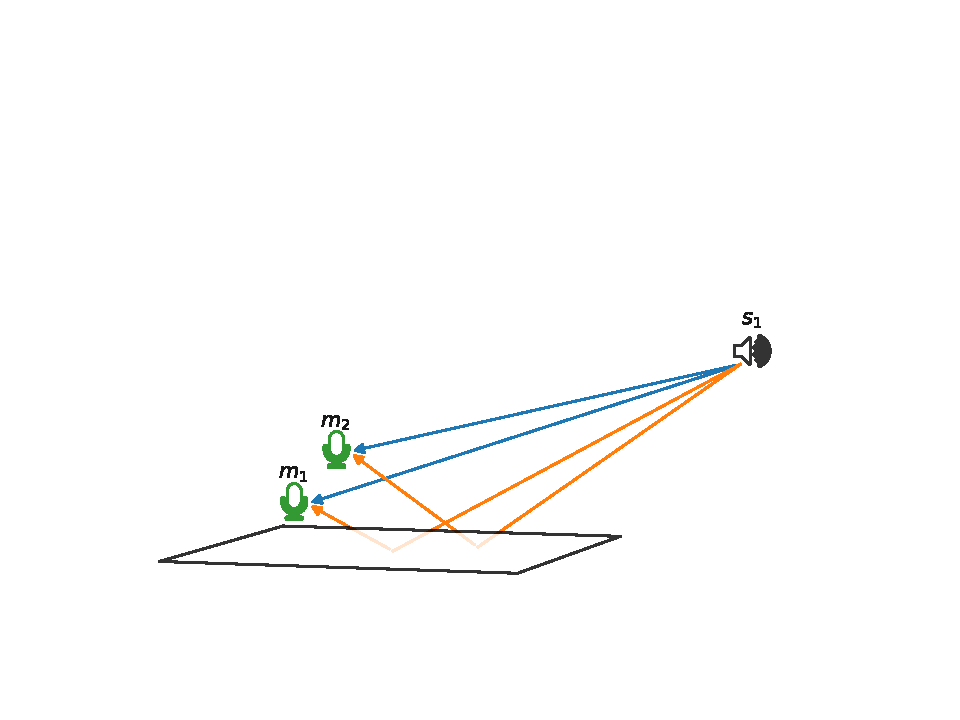
\includegraphics[trim={50 70 50 150},clip,width=\linewidth]{mirage/scene.pdf}
    \captionof{figure}{%
        Typical setup with one sound source recorded by two microphones.
        The illustration shows the direct sound path (blue lines) and the resulting first-order echoes (orange lines).}
    \label{fig:lantern:scene}
}
As a first step, we will use \acp{DNN} to estimate the timings of the first and strongest echo in each channel from stereophonic recordings.
This setup is related to ``table-top'' scenarios, which are commonly encountered in typical home smart audio devices and it is motivated by the echo-aware \acf{SSL} application that will be discussed in~\cref{ch:mirage}.
To this end, we consider the following simple setup: two microphone placed close to a surface, as illustrated in~\cref{fig:lantern:scene}.
The reason why we consider only one microphone pair is that this approach can be generalized to microphone arrays using data-fusion-like techniques.
In fact, by considering all the pairs, it is possible to aggregate their estimation in a second stage.\sidenote{
    An example of such techniques is the \ac{SRP-PHAT}~\citeonly{dibiase2001robust} algorithm used for \ac{SSL}, which uses
    the knowledge of the microphone array geometry to aggregate the contribution of each microphone pair.
}
In the reminder of this chapter, we will discuss how to achieve robust first-echo estimation and how it could be generalized to multiple echoes.

\subsection{Proposed approach}\label{subsec:lantern:simple:mpl}
Our approach is to train a \acp{DNN} on a dataset simulating the considered close-surface scenario.
Under this assumption and the \acf{STFT} signal model presented in~\cref{eq:processing:stft}, we can consider the following simplified model for the \acfp{RTF},
\begin{equation}\label{eq:mirage:rir}
    \FLT_\idxMic[k] = \sum_{\idxEch=0}^{\numEchs=1}  \; \alpha_\idxMic^{(\idxEch)}[k] \; \cste^{- \csti 2 \pi f_k \tau_\idxMic^{(\idxEch)}} \; + \; \varepsilon_\idxMic[k],
\end{equation}
where $\tau_\idxMic^{(\idxEch)}$ and $\alpha_\idxMic^{(\idxEch)}[k]$ are the echoes' times of arrival and amplitudes, respectively.
Here, $f_k$ denotes $k$-th frequency bin and the error term $\varepsilon_i[k]$ collects later echoes, the reverberation tail, diffusion, and noise.
\\As we consider only the first echo per channel, let be $\numEchs=1$.
Given the close-surface scenario, the first echo is the earliest and strongest.

\mynewline
We model the \AER/ problem a multi-target regression problem, namely, the outputs of the model are multiple real-valued parameters.
Following the approaches suggested in~\citeonly{deleforge2015acoustic,gaultier2017vast}, we consider the instantaneous \acf{ILD} and the \ac{IPD} as input features.
As discussed in~\cref{subsec:processing:steering}, the \acfp{ILD} and \acfp{IPD} can be consider as a particular case of \acf{ReTF}.
The \ac{ILD} and \ac{IPD} can be estimated from the \STFT/ of the microphone signals as follows
\begin{equation} \label{eq:mirage:features}
\begin{cases}
    \ild[k]  =& \tfrac{1}{T} \sum_{l=1}^T \log{\abs{\frac{\MIC_2[k,l]}{\MIC_1[k,l]}}}, \\
    \ipd[k]  =& \tfrac{1}{T} \sum_{l=1}^T \frac{\MIC_2[k,l]/ \abs{\MIC_2[k,l]}}{ \MIC_2[k,l] / \abs{\MIC_1[k,l]}},\\
\end{cases}
\end{equation}
where $\MIC_i[k,l]$ is the \ac{STFT} of the $i$-th microphone.
\\More precisely, the input of the network is
\begin{equation*}
    \xi = \klist{ \ild, \kRe\set{\ipd}, \kIm\set{\ipd}}
    ,
\end{equation*}
namely, the concatenation of the above features in all frequencies into a single vector..
Here $\kRe\set{\cdot}$ and $\kIm\set{\cdot}$ denote real and imaginary part operators, respectively.
Note that for the \ac{IPD}, the frequency $k=0$ is discarded because because it always equals 1 for all the frequencies.

\newcommand{\setTDOA}{\ensuremath{\set{\mathtt{TDOA}, \mathtt{iTDOA}, {\mathtt{TDOE}_1}}}}
\mynewline
Initial investigations showed that learning the echoes amplitudes yielded large estimation errors, probably due to the complexity of the task.
Thus, we considered echo timings with respect to the direct-path \ac{TOA} in a reference microphone for the following three main reasons:
first, the origin of time cannot be known in the blind setting;
second, motivated by an application to passive \ac{SSL} discussed in~\cref{ch:mirage}, \acfp{TDOA} can easily converted to angles.
Then, the timings of the first echoes in the two channels can be fully parameterized by the following three quantities:
\begin{equation}
    \begin{cases}
        \tau_\mathtt{TDOA}  &= \tfrac{1}{c} \norm{\positionMicrophone_2 - \positionSource} - \tfrac{1}{c} \norm{\positionMicrophone_1 - \positionSource} = \tau_2^{(0)} - \tau_1^{(0)} \quad[\text{s}],\\
        \tau_\mathtt{iTDOA} &= \tfrac{1}{c} \norm{\mathring{\positionMicrophone}_2 - \positionSource} - \tfrac{1}{c} \norm{\mathring{\positionMicrophone}_1 - \positionSource} = \tau_2^{(1)} - \tau_1^{(1)} \quad[\text{s}],\\
        \tau_{\mathtt{TDOE}_1}  &= \tfrac{1}{c} \norm{\mathring{\positionMicrophone}_1 - \positionSource} - \tfrac{1}{c} \norm{\positionMicrophone_1 - \positionSource} = \tau_1^{(1)} - \tau_1^{(0)} \quad[\text{s}],\\
        \tau_{\mathtt{TDOE}_2}  &= \tfrac{1}{c} \norm{\mathring{\positionMicrophone}_2 - \positionSource} - \tfrac{1}{c} \norm{\positionMicrophone_2 - \positionSource} = \tau_2^{(1)} - \tau_2^{(0)} \quad[\text{s}],
    \end{cases}
\end{equation}
where $\mathring{\positionMicrophone}_i$ denotes the position of the image of the microphone at position $\positionMicrophone_i$ with respect to the reflector.
Note that, since $\tau_{\mathtt{TDOE},2} = \tau_\mathtt{iTDOA} + \tau_{\mathtt{TDOE}, 1} - \tau_\mathtt{TDOA}$, only the first three will be considered.
These three quantities are directly connected to the early parts of the \RIRs/, as illustrated in~\cref{fig:lantern:rirs_tdoa}\marginpar{%
\centering
\footnotesize
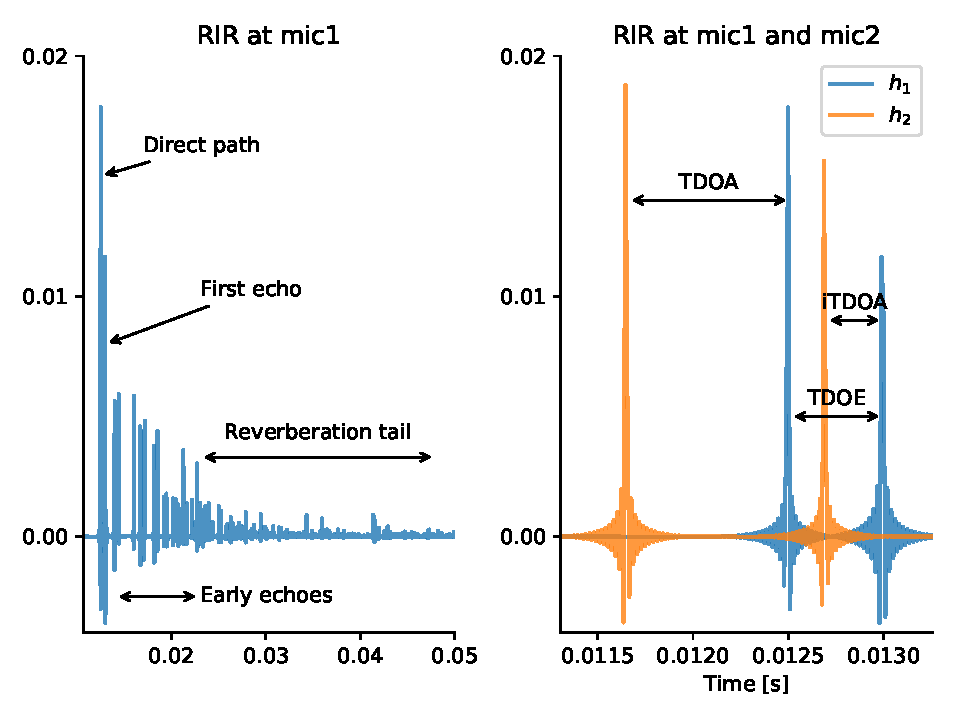
\includegraphics[trim={82mm 0 0 0},clip,width=\linewidth,height=7cm]{mirage/rirs.pdf}
\captionof{figure}{%
    Superposition of two synthetic \acp{RIR} and visualization of time differences of arrival between direct paths (\acs{TDOA}), first echoes (\acs{iTDOA}) and direct path and first echo (\acs{TDOE}).}
\label{fig:lantern:rirs_tdoa}
}. Let $V = \klist{\tau_{\mathtt{TDOA}}, \tau_{\mathtt{iTDOA}}, \tau_{\mathtt{TDOE}_1}}\in\mathbb{R}^3$ be the vector of parameters of interest.
Since it will be useful later, let define $\calV = \setTDOA$ the set of three \textbf{indexes} denoted by \ac{TDOA}, \ac{iTDOA}, \ac{TDOE}.

\mynewline
Since we use \ReTF/-based features to estimate echoes, the proposed approach is dubbed \textit{\acf{LANTERN}}.

\mynewline
While, given the $V$, the early part of the \ac{RTF} is fully defined, the opposite in not.
Therefore, in general, different values of $V$ can yield the same \ac{ReTF} and hence the same \ac{ILD}/\ac{IPD} features.
In particular, this happens when $\tau^{(1)}_1 - \tau^{(0)}_1 = \tau^{(1)}_2 - \tau^{(0)}_2$ for $\idxEch=\set{0,1}$.
That is, \ac{TDOE}s are equal, or equivalently, the \ac{TDOA} is equal to the \ac{iTDOA}.
Geometrically, this correspond to the case where real and image source have the same angle of arrival, which occur in very specific source / array / reflector configurations.
Since this degenerate case is fundamentally unsolvable in the blind setting, we preventively pruned, all the entries with $| \tau_\mathtt{TDOA} - \tau_\mathtt{iTDOA} | < 10^{-6}$ from all the dataset.
In particular, they are removed from the training set so that the training is not affected by these degenerate cases.
Moreover, these are degenerate situations are known to be non-solvable and are not included in the evaluation to not bias the metrics.

\mynewline
Here we use the simple \ac{MLP} architecture described in~\cref{subsec:lantern:mlp}.
This model consists of a $D$-dimensional input layer, a 3-dimensional output layer, and 3 fully connected hidden layers with respective input sizes $500$, $300$, and $50$.
\ac{ReLU} activation functions are used except at the output layer, and each hidden layer has a dropout probability $p_\text{do} = 0.3$ to prevent overfitting.
\\We use the \ac{MSE} loss function for training, that is,
\begin{equation}\label{eq:lantern:mlploss}
    \calL_\theta(V, \hat{V)} = \frac{1}{|\calV|} \sum_{\xi\in\Xi} \sum_{v\in\calV} \powerOf{\tau_{v, \xi} - \hat{\tau}_{v, \xi}}
\end{equation}
where $v$ indexes one of the \acp{TDOA} in $\calV$, $\xi$ denotes a sample index in the mini-batch $\Xi$, and $\theta$ contains the model parameters.

\mynewline
The \acf{nRMSE}\sidenote{
    The \ac{nRMSE} takes values between $0$ (perfect fit) and $\infty$ (bad fit).
    If it is equal to $1$, then the prediction is no better than a constant.
}is taken as validation metric to assess the quality of the estimation $\hat{V}$.
For the vectors $T$ and $\hat{T}$ containing the reference and estimated value for all the sample $\xi$. the \ac{nRMSE} is define as
\begin{equation*}
    \mathtt{nRMSE}(\hat{T}, T) = \frac{\norm{\hat{T} - T}_2}{\norm{T - \mathtt{avg}(T)}_2}
    ,
\end{equation*}
where $\norm{\cdot}_2$ denotes the $\ell_2$ norm and $\mathtt{avg}{\cdot}$ is the average operation over the sample $\xi$.
The network is manually tuned on a validation set to find the best combination of number of hidden layers, layer sizes and $p_\text{do}$.

\subsection{Data, implementation and experimental results}\label{subsec:lantern:simple:mpl:results}
For training and validation of the \ac{MLP} we generate many random, shoe-box room configurations using the software presented in \citeonly{schimmel2009fast}.
This software implements both the \acf{ISM} for simulating reflections and a ray-tracing algorithm for diffusion~\cref{sec:acoustics:simulators}.
Room widths are uniformly drawn at random in $[3, 9]$ m, and heights in in $[2, 4]$ m.
Random source and microphone positions are used, respecting the close-surface scenario.\sidenote{
    A rejection-sampling strategy was used to approximate uniform distributions.
}
In particular, the microphones are at most 30~cm from the close-surface, placed 10~cm from each other, the other walls' (frequency-independent) absorption coefficients are uniformly sampled in $\kintervoo{0.5}{1}$ and the one of the close-surface is sampled in $\kintervoo{0}{0.5}$.
The same realistic diffusion profile \citeonly{gaultier2017vast} is used for all surfaces.
Around $90,000$ \acp{RIR} are generated this way, with a \ac{RT$_{60}$} between $20$~ms and $250$~ms.
\\The \acp{RIR} are convolved with 1 sec of white-noise (wn) with no additional noise.
All signals and \acp{RIR} are sampled at 16~kHz.
The \ac{STFT} is performed on 1024~points with 50\% overlap.
Finally the features are computed as in~\eqref{eq:mirage:features} yielding a vector of size $D = 1534$ for each observation.
\\While we validate the \ac{MLP} on a portion of the dataset in a \textit{holdout} fashion, the test is conducted on 200 new \acp{RIR} convolved with both wn and speech (sp) utterances.
This set is generated similarly to the training and validation sets.
Moreover, the test recordings are perturbed by external white noise at 10~dB \acf{SNR} (wn+n, sp+n).
The speech signals are normalized speech utterances of various lengths (from 1~s to 6~s), randomly selected from the TIMIT corpus.
% A free and open-source Matlab implementation of SRP-PHAT\footnote{\url{http://bass-db.gforge.inria.fr/bss_locate/}} is used to aggregate local angular spectra obtained from the DNN's output.
% The same toolbox is used for the implementation of SPR-PHAT with GCC-PHAT. For the latter method only real pairs are used.
% A sphere sampling with $\ang{0.5}$ resolution and coordinates $\theta \in [-179, 180]$ and $\phi \in [0, 90]$ is used for the DOA search.

\newthoughtpar{Experimental results}
To check the validity of \ac{TDOA} estimation with the proposed \ac{MLP} model, we compare it to a baseline algorithm \acf{GCC-PHAT} (see~\cref{subsec:mirage:1D-SSL}).
\ac{GCC-PHAT} is a popular method for estimating the \ac{TDOA} between two microphone recordings.
It is known to achieve good performance in the case of broadband source signals.
However, it was shown that as soon as the acoustic conditions become challenging due to strong early echoes, high reverberation level, and noise, the method performances decrease~\citeonly{chen2006time}.

\begin{table}[h]
    \begin{sidecaption}[Echo estimation with MIRAGE results]{%
        \acfp{nRMSE} for TDOA estimation using the \ac{MLP} architecture.
    }[tab:lantern:tdoas-aoa]
    \centering
    \footnotesize
    \small
    \begin{tabular*}{\linewidth}{@{\extracolsep{\fill}}lll|cccc@{}}
    \toprule
    &            &         &          & nRMSE           &\\
    &            & Input   &    \ac{TDOA}  	&   \ac{iTDOA} 		 &     \ac{TDOE}   	&\\
    \midrule
    & MIRAGE-MPL      &   wn    & 0.18    & 0.28  & 0.25 	& \\
    & MIRAGE-MPL      &   wn+n  & 0.68    & 0.69  & 0.89 	& \\
    & MIRAGE-MPL      &   sp    & 0.31    & 0.34  & 0.56    & \\
    & MIRAGE-MPL      &   sp+n  & 0.99    & 0.98  & 1.48 	& \\
    & GCC-PHAT    &   wn    & 0.21    & -     & -		& \\
    & GCC-PHAT    &   wn+n  & 0.68    & -     & -		& \\
    & GCC-PHAT    &   sp 	& 0.32    & -     & -		& \\
    & GCC-PHAT    &   sp+n  & 1.38    & -     & -		& \\
    \bottomrule
    \end{tabular*}
    \end{sidecaption}
\end{table}

\mynewline
\ac{TDOA} estimation errors using the proposed approach and \ac{GCC-PHAT} are presented in~\cref{tab:lantern:tdoas-aoa}.
From these results, one can see that training a \ac{MLP} to estimate \acp{TDOA} brings similar performances as \ac{GCC-PHAT} in terms of nRMSE for clean white noise and speech signals.
However, the estimation of \ac{iTDOA} and \ac{TDOE} seems to be a more challenging task for such a simple \ac{MLP} model.
For both the methods, the performance are generally worse on speech signals than on white noise signals, which is due to the spectral sparsity of speech signals.
However, in the noiseless scenario, it is interesting to see that even a simple architecture trained on \ac{ReTF}-based features and broadband data is somehow able to generalize to speech.
Unfortunately, when some external noise is added, the performances of the methods degrade in all the cases.
This is a well-known and expected behavior for \ac{GCC-PHAT}, and for the \ac{MLP} it suggests that noise should also be considered in the training phase.
Nevertheless, our results confirm the possibility of retrieving the strongest echoes from only two-microphone recordings, in the absence of noise.

\section{Robustly learning the first echo}\label{sec:lantern:robust}
The above study was presented in our published work~\citeonly{di2019mirage}.
To overcome the limitations of of our simple \ac{MLP}-based method, we introduced the following three modifications:
\begin{itemize}
    \item use a more elaborate architecture inspired by a state-of-the-art SSL method;
    \item include corrupting noise in the training data;
    \item use a robust loss function which is able to return a level of confidence on the estimations.
\end{itemize}
Motivated by their success, we consider a \ac{CNN} architecture (see~\cref{subsec:lantern:cnn}).
To this end, we inspire from the work of~\citeonly{chakrabarty2017broadband,nguyen2018autonomous} in \ac{SSL}.
\begin{figure}[h]
    \begin{sidecaption}[CNN]{
        Architecture of the proposed deep neural network. Input and output dimensions for each stage are reported. The first dimension is the batch size $B = 200$.
        }[fig:lantern:cnn]
        \centering
        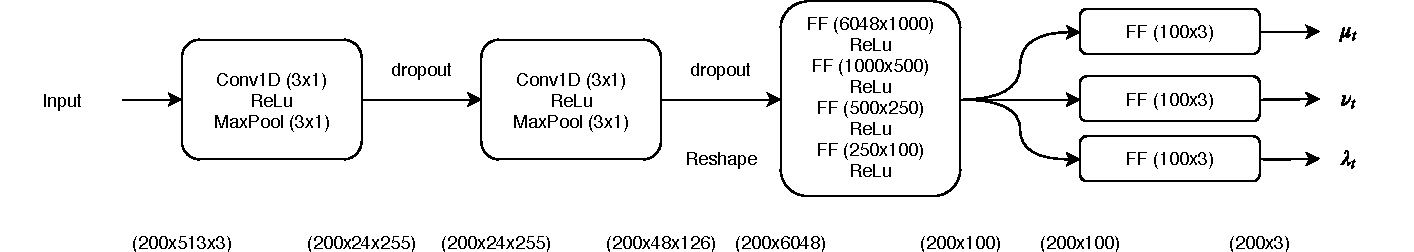
\includegraphics[width=\linewidth]{mirage/cnn.pdf}
    \end{sidecaption}
\end{figure}
As shown in~\cref{fig:lantern:cnn}, the architecture consists of two convolutional modules made of a one-dimensional convolutional layer (Conv1D) followed by max-pooling along frequencies, followed by \ac{ReLU} activation function and batch-normalization.
The second part consists of a cascade of fully connected feed-forward (FF) layers (basically the \ac{MLP} model discussed above).
In order to perform 1D-convolution in the correct (temporal) dimension, we re-arranged the input so that the each of the features $\set{ \ild, \kRe\set{\ipd}, \kIm\set{\ipd}}$ is considered as a channel for the Conv1D.
After each layer, a dropout probability $p_\text{do} = 0.3$ is applied to prevent overfitting.

\mynewline
\subsection{Gaussian- and Student's T-based CNNs}
In the \ac{MLP} model presented in the previous section, the output consisted only in the \acp{TDOA} $V$.
As mentioned earlier, our final goal is to generalize this approach to microphone arrays in a data-fusion-like fashion.
To this end, we need to provide a confidence measure on the estimate.
In our work~\citeonly{di2019mirage}, we proposed to use predicted values and the errors on the validation set as means and variances to build a Gaussian priors ((see~\cref{ch:mirage} for details on this)).
Instead, here, we explicitly modify the \ac{CNN} model to estimated these parameters.
This idea recalls the \acp{MDN} as presented in in \citeonly{bishop1994mixture}, where the output of a neural network parametrizes a Gaussian mixture model.
The rationale behind this design choice is to allow the learning model to assess its prediction quality.
In order to achieve this, both the loss functions and the network outputs need to be modified accordingly.
\newcommand{\xiTheta}{{\xi;\params}}
\newcommand{\sigmaTauv}{\ensuremath{\sigma^2_{v}(\xiTheta)}}
\newcommand{\muTauv}{\ensuremath{\mu_{v}(\xiTheta)}}
\newcommand{\sigmaTau}{\ensuremath{\sigma^2_{v}}}
\newcommand{\muTau}{\ensuremath{\mu_{v}}}
\newcommand{\estSigmaTau}{\ensuremath{\sigma^2_{v}}}
\newcommand{\estMuTau}{\ensuremath{\mu_{v}}}

\newthought{The Gaussian-based loss function} is derived as follows.\marginpar{
    \footnotesize
    The general form of the Gaussian probability density function is
    \begin{equation*}
        \calN\kparen{x; \mu, \sigma^2} = \frac{1}{\sqrt{2\pi \sigma^2}}
                                         \cste^{- \frac {1}{2} \kparen{\frac{x-\mu}{\sigma }}^2}
        .
    \end{equation*}
} First, we modify the network to return means and variances, namely
$V_{\calN} = \set{\muTauv, \sigmaTauv}_v$ for $v = \setTDOA$.
Moreover, we assume that the posterior probability of observing $\tau_v$ for $v \in \setTDOA$, given the observation $\xi$ in the mini-batch $\Xi$, follows a Gaussian distribution, namely
\begin{equation}
    p(\tau_v \mid  \xi ; \params) \sim \calN\kparen{\tau_v; \muTauv, \sigmaTauv}
    .
\end{equation}
From now on, we omit the dependency on $(\xiTheta)$ for the sake of clarity.
\\Finally, the corresponding training loss function is the negative the negative log-posterior probability over the batch $\Xi$, that is,
\begin{equation}\label{eq:lantern:gausslog}
    \begin{aligned}
        \calL_{\params}^{\calN}(V, \hat{V)}
                    &= - \log \prod_{\xi\in\Xi}\prod_{v\in\calV} p(\tau_v|\xi ; \params) \\
                    &\stackrel{c}{=} \frac{1}{\kvbar{\calV}}
                    \sum_{\xi\in\Xi} \sum_{v\in\calV}
                    \log{\estSigmaTau}
                    + \frac{\powerOf{\tau_v - \estMuTau}}{\estSigmaTau}
    \end{aligned}
    ,
\end{equation}
where $\stackrel{c}{=}$ denotes equivalence up to a constant.
\\Hence, for a given input $\xi$, the network attempts to find mean and variance parameters maximizing the \textit{a posteriori} probability of \acp{TDOA} according to the considered Gaussian model.
The means are then used as \ac{TDOA} estimates, while variances can be seen as a measure of uncertainty from the model.
Hereafter we denote by $\hat{V}_{\calN}$ the set of 6 network outputs.
\\This approach can then be generalized to other this of distributions.
For instance, we can consider a Student's \textit{t}-distribution, which is more robust to outliers, due to its heavy-tailed nature.
Using this distribution has already been proposed in the context of binaural \ac{SSL}, \eg/, in~\citeonly{zohny2014modelling,deleforge2016rectified}.

\newthought{The Student's \textit{t}-based loss function}
\marginpar{
    \footnotesize
    The general form of the Student's \textit{t} probability density function is
    \begin{equation*}
        \calT(x; \mu, \lambda, \nu) = \frac{\Gamma(\frac{\nu+1}{2})} {\sqrt{\nu\pi}\,\Gamma(\frac{\nu}{2})} \left(1+\frac{x^2}{\nu} \right)^{\!-\frac{\nu+1}{2}}
        ,
    \end{equation*}
    where $\Gamma(n)=(n-1)!$ is the Gamma function, defined for positive integers.
} can be derived similarly as the Gaussian case assuming a \textit{t}-distribution posterior on the prediction.
% \newcommand{\nuTauv}{\ensuremath{\nu^2_{\tau_v}(\xiTheta)}}
% \newcommand{\lambdaTauv}{\ensuremath{\lambda^2_{\tau_v}(\xiTheta)}}
% \begin{equation}
%     p(\tau_v \mid  \xi ; \theta) \sim \calT\kparen{\tau_v; \muTauv, \lambdaTauv, \nuTauv}
%     .
% \end{equation}
% \begin{equation}
The corresponding negative log-posterior probability over the batch $\Xi$ now writes
\begin{equation}
    \begin{split}
    \ \calL_{\params}^{\calT}(V, \hat{V)} =
                         \sum_{\xi\in\Xi} \sum_{v\in \calV}
                        &    \dfrac{1}{2} \log (\nu_v\pi_v)
                           + \dfrac{1}{2} \log(\lambda_v^2)
                           - \log  \Gamma \left( \dfrac{\nu_v+1}{2} \right)\\
                        &  + \log  \Gamma \left( \dfrac{\nu_v}{2} \right)
                           + \dfrac{\nu_v+1}{2} \log \left( 1  + \dfrac{\powerOf{\mu_v - \tau_v)}}{\nu_v \lambda_v^2} \right)\\
    \end{split}
\end{equation}
where $\Gamma$ is the Gamma function.
Similarly to the Gaussian case, for a given input, the network returns the 3 parameters of 3 \textit{t}-distributions ($\mu_v, \nu_v, \lambda_v$), one for each index $v\in\calV$.
The set of 9 network outputs is denoted by $\hat{V}_{\calT}$.

\subsection{Experimental results}\label{subsec:lantern:simple:cnn:results}
In order to validate the proposed approach, it is compared to the vanilla \ac{MLP} model proposed above in the previous section.
Rather than training on noise-less observation, we consider microphone recordings featuring background noise.
To this end, we perturb the observed microphone signals with \acf{AWGN}, leading to \ac{SNR} values uniformly distributed in $[0, 30]$~dB.
Meanwhile, the test set includes observations featuring \ac{SNR} levels of 0, 10, or 20~dB.
The protocol to generate the observations and the feature extraction step are the same (\cref{subsec:lantern:simple:mpl:results}), but the investigation is restricted to broadband source signals (white noise) only.
Informal test on speech data yielded to 3.3 times larger errors respect to noise signals and close to random.
One of the main reason is due to the missing frequencies in speech spectrum.
Such spectral holes lead to zeros and poles in the computation of the audio features \ac{ILD} and \ac{IPD} (see~\cref{subsec:processing:rtf}).
Alternative technique are currently investigates to overcome this limitation, \eg/, robust \ac{ReTF} estimator or \ac{DNN} handling missing data.
Finally, the network is manually tuned on a validation set in order to find the best combination of number of hidden layers and their sizes, which led to the model in~\cref{fig:lantern:cnn}.
\begin{figure}[h]
    \begin{sidecaption}[]{%
        Normalize root mean squared error (the lower, the better) for \ac{TDOA} estimation using the proposed architectures on white noise source signals.
    }[fig:lantern:snr10]
    \centering
    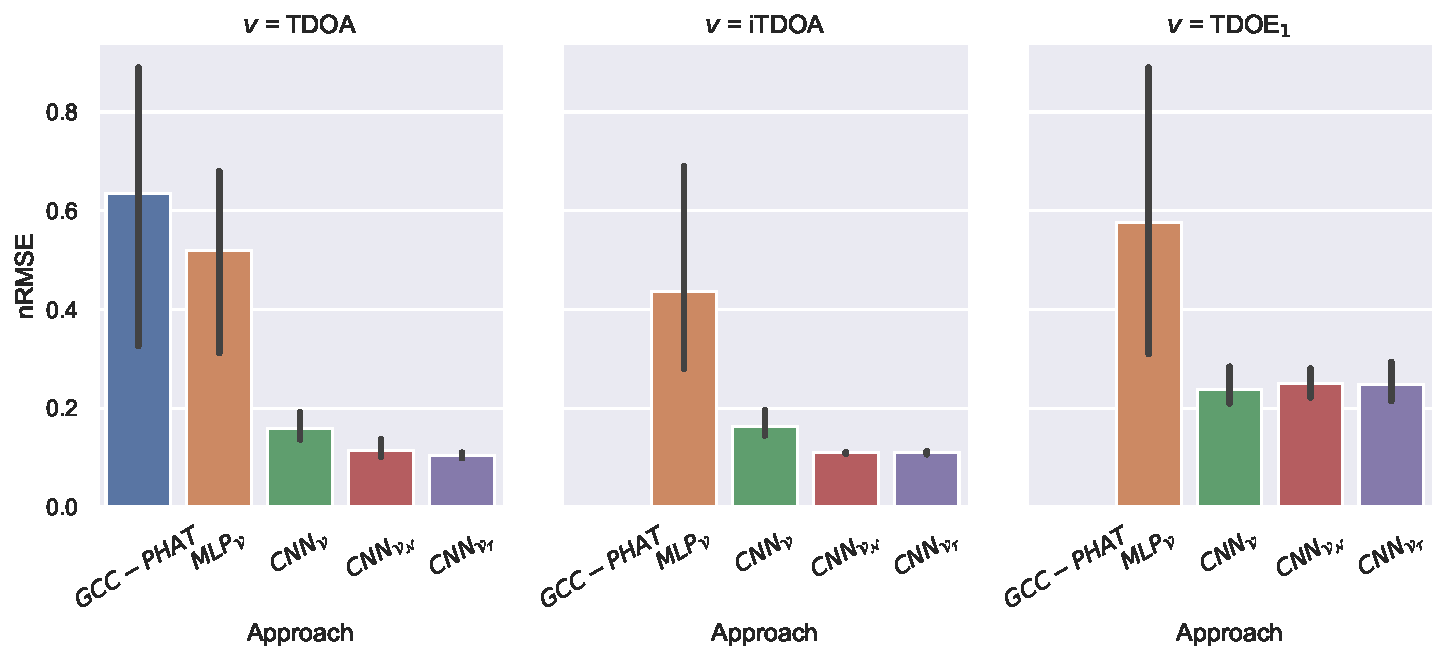
\includegraphics[trim={0 9mm 0 0},clip,width=\linewidth]{lantern/snr10.pdf}
    \end{sidecaption}
\end{figure}
\begin{figure}[h]
    \begin{sidecaption}[]{%
        Normalize root mean squared error (the lower, the better) for \ac{TDOA} estimation using the proposed architectures for different \ac{SNR} levels on white noise source signals.
    }[fig:lantern:snr]
    \centering
    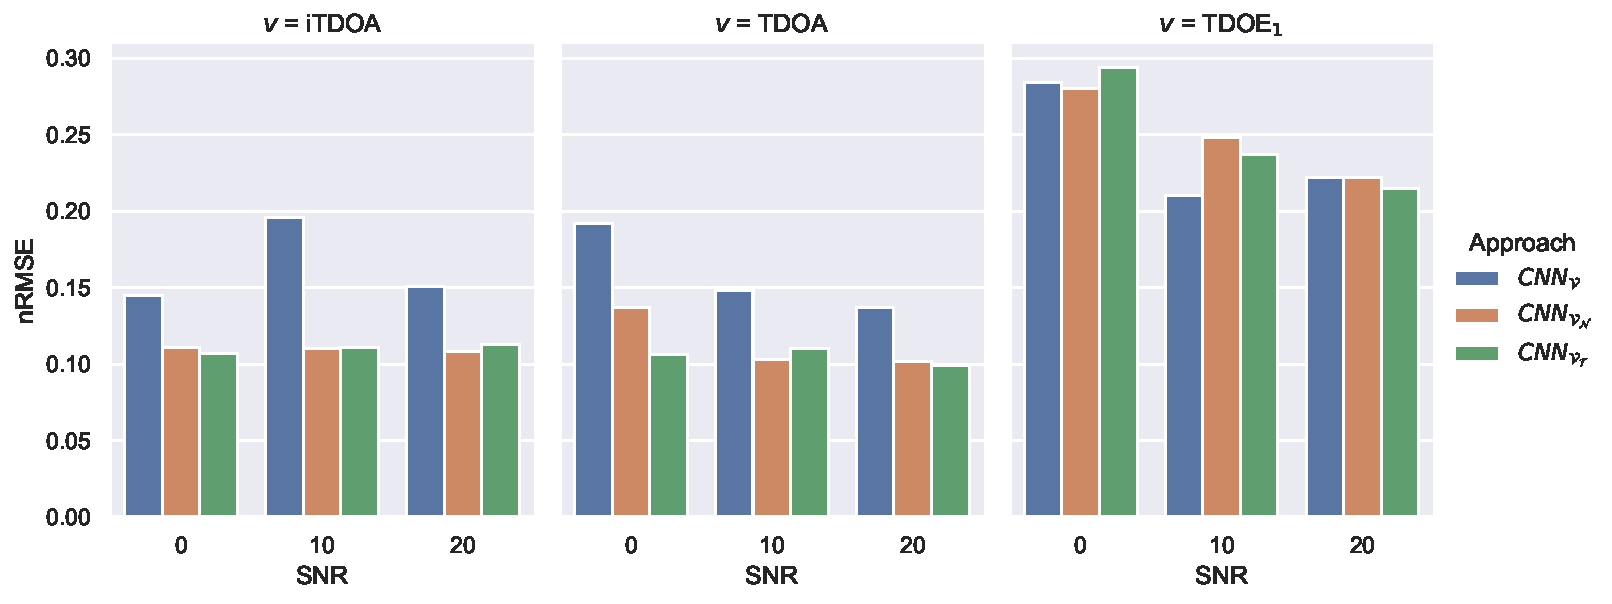
\includegraphics[width=\linewidth]{lantern/snr.pdf}
    \end{sidecaption}
\end{figure}

\noindent \cref{fig:lantern:snr10} shows the performances of the proposed models $\mathtt{CNN}_{\calV}$, $\mathtt{CNN}_{\calV_\calN}$ and $\mathtt{CNN}_{\calV_\calT}$
with respect to $\mathtt{MLP}_{\calV}$ and the baseline $\mathtt{GCC-PHAT}$ for the task of estimating \ac{TDOA}, \ac{iTDOA} and \ac{TDOE}.
Again we report the performances in terms of the \ac{nRMSE} computed on test samples.
It can be seen that the proposed modifications (\ac{CNN} architecture, robust loss function, and considering noise in training) yield considerable improvement in performances, compared to the vanilla and baseline methods.
In particular, the new methods are more robust to noise, as indicate by error bars.
While both $\mathtt{CNN}_{\calV_\calN}$ and $\mathtt{CNN}_{\calV_\calT}$ outperform the $\mathtt{CNN}_{\calV}$ for \ac{TDOA} and \ac{iTDOA} estimation, there is no significant\sidenote{Significance assessed with a t-test for $p<0.05$.} difference between the three of them for \ac{TDOE} estimation.
\\Deeper insights about this can be gathered from~\cref{fig:lantern:snr}, where performances are reported for the different \ac{SNR} levels considered in the test.
These results suggest that using a simple \ac{MSE}-based loss function leads to errors more sensitive to external noise.
In general, there does not seem to be a significant difference between using a Gaussian distribution or a Student's \textit{t}-distribution at the network's output in our experiments.
Nevertheless, the choice of modeling the output of the network according to different distributions may lead to differences at the data-fusion step, as will be explored in~\cref{ch:mirage}.

\section{Conclusion}\label{sec:lantern:conclusion}
This chapter presented an attempt at using deep learning models to learn the complex mapping from stereophonic recordings to echoes' timings.
As part of a first investigation, we considered a simple, yet common scenario where two microphones are placed close to a reflective surface and attend a to a single sound source.
The problem is then restricted to estimating the the relative delays between the direct path and the first echo timings within the two channels.
This simplification is motivated by an application to echo-aware \ac{SSL}, which will be presented in~\cref{ch:mirage}.
\\We studied two standard \ac{DNN} architectures, which are trained in \textit{virtually supervised} fashion on data generated by an acoustic simulator.
Finally, we discuss three ways to improving such performances, \ie/, training on noisy data, using a \ac{CNN}-based architecture, and using robust loss functions.
\\The investigation so far was limited to microphone pairs.
Taking inspiration from data-fusion approaches, in chapter~\cref{ch:mirage}, we will propose to aggregate the contributions of multiple pairs to improve the final estimation.

\mynewline
A natural follow-up of this work could consider the following directions.
\begin{itemize}
    \item The first one would be a generalization to more reflections, which is far from being trivial.
    Informal investigations spanned different training paradigms, such as, \textit{curriculum learning}~\citeonly{bengio2009curriculum}, \textit{teacher-student learning}~\citeonly{tu2019speech}, where the network is iterative trained to estimate more and more echoes.
    Another idea would be to use a collection of \acp{DNN}, each pre-trained for single echo estimation.
    \item Due to severe drops of performance observed using speech signals, we could consider more robust audio features (\eg/, \ReTF/ using state-of-the-art \ReTF/ estimators) or
    \ac{DNN} architectures designed to handle missing input data.
    \item Finally, another interesting direction would be to use physics-driven neural networks as explored in~\citeonly{nabian2020physics,rao2020physics,jin2020physics},
    where physics-based layers or physically-motivated regularizers are implemented to facilitate the learning.
\end{itemize}

% \begin{table}[ht!]
%     \begin{sidecaption}[Echo estimation with MIRAGE results]{%
%         Normalize root mean squared error for TDOA estimation and mean angular error in ${}^\circ$ (with accuracies ($\%$))
%         for AOA estimation with $\ang{10}$ and $\ang{20}$ angular tolerance.
%     }[tab:mirage:tdoas-aoa]
%     \centering
%     \footnotesize
%     %\scriptsize
%     \begin{tabular}{cl|ccc|cc}
%     \toprule
%                 &         &          & nRMSE        &                   &\multicolumn{2}{c}{ACCURACY}  \\
%                 & Input   &    \scriptsize{TDOA}  	&   \scriptsize{iTDOA} 		 &     \scriptsize{TDOE} 		 & $\theta<\ang{10}$ &  $\theta<\ang{20}$ \\
%     \midrule
%     MIRAGE      &   wn    & 0.18    & 0.28  & 0.25 	& 4.10 (77)	& 5.97 (97) \\
%     MIRAGE      &   wn+n  & 0.68    & 0.69  & 0.89 	& 5.00 (26)	& 9.89 (54) \\
%     MIRAGE      &   sp    & 0.31    & 0.34  & 0.56  & 4.83 (63)	& 7.26 (82) \\
%     MIRAGE      &   sp+n  & 0.99    & 0.98  & 1.48 	& 4.60 (16)	& 9.88 (35) \\
%     GCC-PHAT    &   wn    & 0.21    & -     & -		& 4.22 (81) & 6.19 (97) \\
%     GCC-PHAT    &   wn+n  & 0.68    & -     & -		& 4.03 (65) & 5.34 (83) \\
%     GCC-PHAT    &   sp 	  & 0.32    & -     & -		& 4.08 (82) & 5.34 (97) \\
%     GCC-PHAT    &   sp+n  & 1.38    & -     & -		& 4.70 (19) & 8.38 (32) \\
%     \bottomrule
%     \end{tabular}
%     \end{sidecaption}
% \end{table}